\documentclass{bredelebeamer}

% Customs:
\usepackage[utf8]{inputenc}
\usepackage{amsmath,amsfonts,amssymb,graphicx}
\usepackage[document]{ragged2e}
\usepackage[Euler]{upgreek}

% Define mathbfit
\DeclareMathAlphabet{\mathbfit}{OML}{cmm}{b}{it}
\DeclareMathAlphabet{\mathbfsf}{\encodingdefault}{\sfdefault}{bx}{n}

\usepackage[backend=biber]{biblatex}
\addbibresource{ref.bib}

% Setting graphics path
\graphicspath{{./rsc/}{./rsc/pdf/}{./rsc/svg/}{./rsc/image/}}

% Define operators
\DeclareMathOperator*{\argmax}{arg\,max}
\DeclareMathOperator*{\argmin}{arg\,min}
\DeclareMathOperator*{\minimize}{Minimize}
\DeclareMathOperator*{\maximize}{Maximize}

% Define textbfit
\makeatletter
\DeclareRobustCommand\bfseriesitshape{
  \not@math@alphabet\itshapebfseries\relax
  \fontseries\bfdefault
  \fontshape\itdefault
  \selectfont
}
\makeatother
\DeclareTextFontCommand{\textbfit}{\bfseriesitshape}

\usefonttheme[onlymath]{serif}

%%%%%%%%%%%%%%%%%%%%%%%%%%%%%%%%%%%%%%%%%%%%%%%% META DATA start

\title[ML Basics]{Spares Kernel Machines}
% Titre du diaporama

\subtitle{A self-study metarials for PRML~\cite{bishop:2006:PRML}}
% Sous-titre optionnel

\author{Jisung Lim\inst{1}}
% The \inst {...} command displays the member's affiliation.
% If there are several speakers: Marcel Dupont \inst {1}, Roger Durand
% \inst {2} Simply add another institute on the model below.

\institute[Yonsei]
{
  \inst{1}%
  B.S. Candidate of Industrial Engineering\\
  Yonsei University, South Korea.
}

\date{8th February, 2017}
% Optional. The date, usually the day of the conference.

\subject{Sparse Kernel Machines 1, SVM.}
% This is used in the pdf metadata

\logo{
  \begin{tikzpicture}
    \pgfmathsetmacro{\myopacity}{0.25}
    \node[opacity=\myopacity] {
      
\includegraphics[scale=0.08]{yonsei_emblem.png}
      
\includegraphics[scale=0.08]{yonsei_logo_text.png}
    };
  \end{tikzpicture}
}

%%%%%%%%%%%%%%%%%%%%%%%%%%%%%%%%%%%%%%%%%%%%%%%% META DATA end

%%%%%%%%%%%%%%%%%%%%%%%%%%%%%%%%%%%%%%%%%%%%%%%% DOCUMENT start

\begin{document}

%%%%%%%%%%%%%%%%%%%%%%%%%%%%%%%%%%%%%%%%%%%%%%%%%%%%%%%%%%% TITLE PAGE

\begin{frame}
  \titlepage
\end{frame}

\printbibliography
%%%%%%%%%%%%%%%%%%%%%%%%%%%%%%%%%%%%%%%%%%%%%%%%%%%%%%%%%%% SUMMARY

\begin{frame}{Summary}
  \tableofcontents
  % Option to add option [pausesections]
\end{frame}

%%%%%%%%%%%%%%%%%%%%%%%%%%%%%%%%%%%%%%%%%%%%%%%%%%%%%%%%%%%%%%%%%%%%%
\section{Introduction}

\subsection{Kernel Method (Review)}
\begin{frame}{Kernel Method (Review)}
\textbf{Dual Representation} \\
  \begin{enumerate}
    \item Many linear models can be reformulated in terms of a \textbf{dual
          representation.}
    \item Kernel function $k(\mathbfit{x},\mathbfit{x}')$ arises naturally. (at
          the same time hide basis term).
    \begin{equation}
      \begin{split}
        y(\mathbfit{x}_{\textrm{new}})
        &= \mathbfit{w}^T \boldsymbol{\phi}(\mathbfit{x}_{\textrm{new}})
        = {\boldsymbol{\phi}(\mathbfit{x}_{\textrm{new}})}^T {(\lambda\mathbf{I} + \boldsymbol{\Phi}^T \boldsymbol{\Phi})}^{-1} \boldsymbol{\Phi}^T \mathbfsf{t} \\
        &= \mathbfit{a}^T \boldsymbol{\Phi} \boldsymbol{\phi}(\mathbfit{x}_{\textrm{new}})
        = {\mathbfit{k}(\mathbfit{x}_{\textrm{new}})}^T {(\mathbf{K} + \lambda \mathbf{I})}^{-1} \mathbfsf{t}
      \end{split}
    \end{equation}

  \end{enumerate}

  \textbf{Constructing Kernel} \\
  \begin{enumerate}
    \item From basis function (or feature space) \\
          (ex) $k(\mathbfit{x}_n,\mathbfit{x}_m) = \boldsymbol{\phi}(\mathbfit{x}_n)
          \boldsymbol{\phi}(\mathbfit{x}_m) / \alpha$
    \item Directly (Should be followed by validation step)
    \item Build them out of simpler one
  \end{enumerate}

  \textbf{Gaussian Process} \\
  \begin{enumerate}
    \item Not $\mathbfit{w}$, now $\mathbfit{y}_n$.
    \item Kernel function arise in covariance matrix $\mathbf{K}$
    \item Pros: Can consider infinite number of basis function.
    \item Cons: Computationally expensive, it requires computations $O(N^3)$ (instead
          of $O(M^3)$), for each new input.
  \end{enumerate}
\end{frame}

\subsection{Sparse Kernel Machines}
\begin{frame}{Sparse Kernel Machines}
  We will look at kernel-based algorithms that have \textbfit{sparse solutions}.

  \textbf{Sparse Kernel Machine}
  \begin{itemize}
    \item Predictions for new inputs depend only on the kernel function
          evaluated at a \textbf{``subset of the training data points.''}
          (Less expensive)
    \item We shall look at SVM (Supported Vector Machines) and RVM (Relevance Vector Machines).
  \end{itemize}

  \textbf{Support Vector Machine}
  \begin{itemize}
    \item Sparse Kernel Machine with deterministc approach. (Non-probabilistic)
    \item Determine model parameters solving convex optimization problem.
          (Local opt. = Global opt.)
    \item Popular for solving problems in classification, regression
          and novelty detection.
  \end{itemize}

  \textbf{Relevance Vector Machine}
  \begin{itemize}
    \item Based on a Bayesian formulation
    \item Provides posterior probabilistic outputs
    \item Typically much sparser solution than the SVM.
  \end{itemize}
\end{frame}

\subsection{Convex optimization and KKT conditions}
\begin{frame}{Convex optimization and KKT conditions (1)}
  \textit{Primal Problem}
  \begin{equation}
    \begin{gathered}
      \mathbfit{x}^* = \argmin_{\mathbfit{x}} f(\mathbfit{x}) \\
      \textrm{where} \\
      \mathbfit{h}(\mathbfit{x}) = \mathbf{0} \\
      \mathbfit{g}(\mathbfit{x}) \leq \mathbf{0} \\
      \mathbfit{x} \geq \mathbf{0}
    \end{gathered}
  \end{equation}


  \textit{Dual problem}
  \begin{equation}
    \begin{gathered}
      (\boldsymbol{\lambda}^*,\boldsymbol{\mu}^*)
      = \argmax_{\boldsymbol{\lambda},\boldsymbol{\mu}} \tilde{L}(\boldsymbol{\lambda},\boldsymbol{\mu})
      = \argmax_{\boldsymbol{\lambda},\boldsymbol{\mu}} \inf_{\mathbfit{x}} L(\mathbfit{x}, \boldsymbol{\lambda}, \boldsymbol{\mu}) \\
      \textrm{where} \\
      \boldsymbol{\lambda} \geq \mathbf{0}
    \end{gathered}
  \end{equation}
\end{frame}

\begin{frame}{Convex optimization and KKT conditions (2)}
  \textit{KKT multipliers}
  \begin{equation}
    L(\mathbfit{x}, \boldsymbol{\lambda}, \boldsymbol{\mu})
    = f(\mathbfit{x}) + \boldsymbol{\lambda}^T \mathbfit{g}(\mathbfit{x})
    + \boldsymbol{\mu}^T \mathbfit{h}(\mathbfit{x})
  \end{equation}

  \textit{KKT conditions}
  \begin{equation}
    \begin{split}
      \textrm{Stationarity: }
      & \nabla_{\mathbfit{x}, \boldsymbol{\lambda}, \boldsymbol{\mu}}
      L(\mathbfit{x}, \boldsymbol{\lambda}, \boldsymbol{\mu})
      = \mathbf{0} \\
      \textrm{primal feasible: }
      & \mathbfit{g}(\mathbfit{x}) \leq \mathbf{0} \\
      & \mathbfit{h}(\mathbfit{x}) = \mathbf{0} \\
      \textrm{dual feasible: }
      & \boldsymbol{\lambda} \geq \mathbf{0} \\
      \textrm{complementary slackness: }
      & \boldsymbol{\lambda}^T \mathbfit{g}(\mathbfit{x}) = \mathbf{0}
    \end{split}
  \end{equation}
\end{frame}

\section{SVM; Introduction}
\subsection{Model setting}
\begin{frame}{Model Setting}
  \begin{itemize}
    \item Let's begin with two-class classification problem using linear models of the form
    \begin{equation}
      \begin{gathered}
        y(\mathbfit{x}) = \mathbfit{w}^T \boldsymbol{\phi} (\mathbfit{x}) + b \\
        \textrm{where} \\
        \boldsymbol{\phi} (\mathbfit{x})\textrm{: finite, fixed feature space} \\
        b\textrm{: bias parameter}
      \end{gathered}
    \end{equation}
    \item The training data set comprises $N$ observations which is given by
    \begin{equation}
      {\{ (\mathbfit{x}_1, t_1), \ldots, (\mathbfit{x}_N, t_N) \}}
      \quad \textrm{where} \quad t_n \in {\{-1, 1\}}
    \end{equation}
    \item We assume, for the moment, that theg training data set is \textbfit{linearly
    separable} in feature space.
    \item In linearly separable setting, we can deterimine $y(\mathbfit{x})$
          exactly satisfying
    \begin{equation}
      y(\mathbfit{x}) \left\{
      \begin{array}{ll}
        > 0 \quad & \textrm{if} \quad t_n = 1 \\
        < 0 \quad & \textrm{if} \quad t_n = -1
      \end{array}
      \right.,
    \end{equation}
    so that $|y(\mathbfit{x})| = t_n y(\mathbfit{x})$.
  \end{itemize}
\end{frame}

\subsection{Maximum Margin Classifiers}
\begin{frame}{Maximum Margin Classifiers (1)}
  The support vector machine approaches this problem through the concept of the
  \textbfit{margin}, which is defined to be the smallest distance between the
  decision boundary and any of the samples.
  \begin{itemize}
    \item \textbfit{Perpendicular distance} between a point $\mathbfit{x}$ and a hyperplane
    $y(\mathbfit{x}) = 0$ is given by
    \begin{equation}
      \frac{|y(\mathbfit{x})|}{||\mathbfit{w}||}
      = \frac{t_n (\mathbfit{w}^T \boldsymbol{\phi} (\mathbfit{x}) + b)}{||\mathbfit{w}||},
    \end{equation}
    since $y(\mathbfit{x}) = \mathbfit{w}^T \boldsymbol{\phi} (\mathbfit{x}) + b$ and
    $|y(\mathbfit{x})| = t_n y(\mathbfit{x})$.
    \item \textbfit{Margin} defined to be the smallest perpendicular distance is given  by
    \begin{equation}
      \min_{n}
        \left\{
          \frac{t_n (\mathbfit{w}^T \boldsymbol{\phi} (\mathbfit{x}) + b)}{||\mathbfit{w}||}
        \right\}
    \end{equation}
    \item We wish to optimize the parameters $\mathbfit{w}$ and $b$ in order to
    \textbfit{maximize the margin}.
    \begin{equation}
      \argmax_{\mathbfit{w}, b}
      \left\{
        \frac{1}{||\mathbfit{w}||} \min_{n}
          \left[
            t_n (\mathbfit{w}^T \boldsymbol{\phi} (\mathbfit{x}) + b)
          \right]
      \right\}
    \end{equation}
    Solving this problem directly would be vary challenging, so we will use some
    technique in next slide.
  \end{itemize}
\end{frame}

\begin{frame}{Maximum Margin Classifiers (2)}
  \begin{itemize}
    \item Rescale $\mathbfit{w}$ and $b$ by same ratio ($t_n y(\mathbfit{x}) /
    ||\mathbfit{w}||$ unchanged) to fix the value of the numerator of the margin
    \begin{equation}
      t_n (\mathbfit{w}^T \boldsymbol{\phi} (\mathbfit{x}) + b) = 1,
    \end{equation}
    so that all data points will satisfies \textbfit{the constraints}
    \begin{equation}
      t_n (\mathbfit{w}^T \boldsymbol{\phi} (\mathbfit{x}) + b) \geq 1 \quad \forall n.
    \end{equation}

    \item Hence we get more simplified optimization problem, given by
    \begin{equation}
      \argmax_{\mathbfit{w}, b} \frac{1}{||\mathbfit{w}||}
       = \argmin_{\mathbfit{w}, b} \frac{1}{2} {||\mathbfit{w}||}^2
    \end{equation}

    \item Since this problem is convex optimization, we will use KKT conditions
          and solve dual problem. First, the KKT multiplier is given by
    \begin{equation}
      L(\mathbfit{w}, b, \mathbfit{\mathbfit{a}})
      = \frac{1}{2} {||\mathbfit{w}||}^2 - \mathbfit{a}^T (\mathbfsf{y} - \mathbf{1}_N)
    \end{equation}

  \end{itemize}
\end{frame}

\begin{frame}{Maximum Margin Classifiers (3); $\mathbfit{a}$}
  \begin{itemize}
    \item Following equations are satisfied by stationarity of KKT conditions
    \begin{equation}
        \mathbfit{w} = \sum_{n=1}^N a_n t_n \boldsymbol{\phi}(\mathbfit{x}_n)
        \quad \textrm{and} \quad
        0 = \sum_{n=1}^N a_n t_n,
    \end{equation}
    so that we get dual problem, given by
    \begin{equation}
      \begin{gathered}
        \argmax_{\mathbfit{a}}
        \left[
        \tilde{L}(\mathbfit{a}) = \sum_{n=1}^{N} a_n
        - \frac{1}{2} \sum_{n=1}^{N}\sum_{m=1}^{N} a_n a_m t_n t_m k(\mathbfit{x}_n, \mathbfit{x}_m)
        \right]\\
        \textrm{where} \\
        \mathbfit{a} \geq \mathbf{0} \quad \textrm{and} \quad
        \mathbfit{a}^T \mathbfsf{t} = 0
      \end{gathered}
    \end{equation}
    \item For a fixed set of basis functions whose number $M < N$, dual problem
    appears much more expensive. However, it allows the model to be
    \textbfit{reformulated using kernels}, and so the maximum margin
    classifier can be applied efficiently to feature spaces whose
    dimensionality exceeds the number of data points, including
    \textbfit{infinite feature space}.
  \end{itemize}
\end{frame}

\begin{frame}{Maximum Margin Classifiers (4); support vectors}
  \begin{itemize}
    \item In order to classify new data points using the trained model, we
    evaluate a prediction function based on kernel which is given by
    \begin{equation}
      y(\mathbfit{x})
      = \mathbfit{w}^T \boldsymbol{\phi}(\mathbfit{x}) + b
      = \sum_{i=1}^{N} a_n t_n k(\mathbfit{x}, \mathbfit{x}_n) + b
    \end{equation}
    since $\mathbfit{w} = \sum_{n=1}^N a_n t_n \boldsymbol{\phi}(\mathbfit{x}_n)$.
    \item For the equation (18), we can find $\mathbfit{a}$ solving the dual problem.
    Before we evalute $b$, we will use KKT condtions to make the model sparser.
    The KKT conditions is given by
    \begin{equation}
      \begin{split}
        a_n &\geq 0 \quad \forall n \\
        t_n y(\mathbfit{x}_n) - 1 &\geq 0 \quad \forall n \\
        a_n {(t_n y(\mathbfit{x}_n) - 1)} &= 0 \quad \forall n,
      \end{split}
    \end{equation}
    i.e., for every sample point, $a_n = 0$ or $t_n y(\mathbfit{x}_n) - 1 = 0$.
  \end{itemize}
\end{frame}

\begin{frame}{Maximum Margin Classifiers (4); support vectors}
  \begin{itemize}
    \item In equation (18), the point $(\mathbfit{x}_n, t_n)$ plays no role in
    making prediction if $a_n = 0$. We call the remaining data points \textbfit{support vectors},
    which satisfies $t_n y(\mathbfit{x}_n) = 1$, so that lie on the maximum
    margin hyperplanes in feature space.
    \item The origin of sparsity in the SVM is that the maximum margin hyperplain
    is can be defined only by the location of the support vectors.
  \end{itemize}
  \begin{figure}
  \centering
  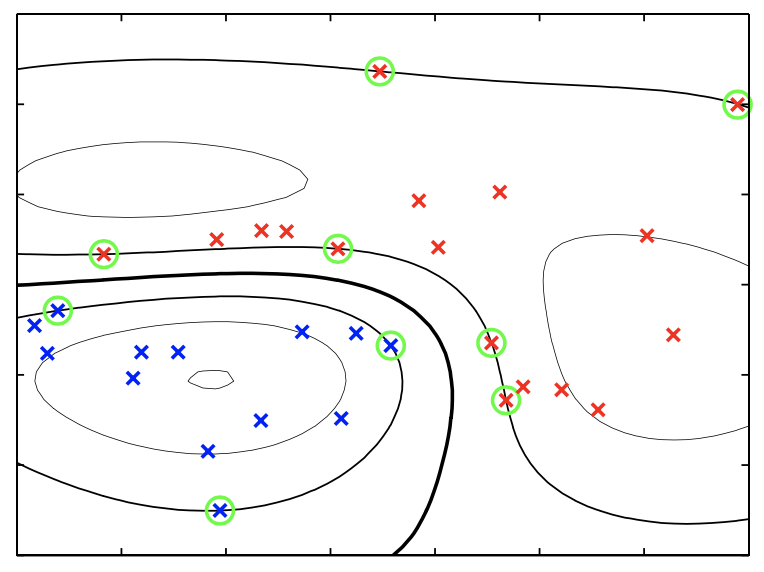
\includegraphics[scale=0.35]{svm_support_vectors.png}
  \caption{
    Contours of constant $y(x)$ obtained from a support vector machine having a
    Gaussian kernel function.
  }
  \end{figure}
\end{frame}

\begin{frame}{Maximum Margin Classifiers (5); $b$}
  We've found $\mathbfit{a}$. Now, we can then determine the value of the
  threshold parameter $b$.
  \begin{itemize}
    \item From $t_n y(\mathbfit{x}_n) = 1$
    \begin{equation}
      t_n \left(
        \sum_{m\in\mathcal{S}} a_m t_m k(\mathbfit{x}_n, \mathbfit{x}_m) + b
      \right) = 1
    \end{equation}
    Where $\mathcal{S}$ denote the set of indices of the support vectors.
    \item Multiply through by $t_n$, make use of $t_n^2 = 1$, and then average
          over every support vector for numerical stability.
    \begin{equation}
      b = \frac{1}{N_\mathcal{S}}
      \sum_{n \in \mathcal{S}}\left(
      t_n - \sum_{m\in\mathcal{S}} a_m t_m k(\mathbfit{x}_n, \mathbfit{x}_m)
      \right)
    \end{equation}
    where $N_\mathcal{S}$ is the cardinality of $\mathcal{S}$.
    \item We can express the maximum margin classifier in terms of the minimization
    of an error function, with a simple quadratic regularizer
    \begin{equation}
      \begin{gathered}
        \sum_{n=1}^N E_{\infty}(y(\mathbfit{x}_n)t_n - 1) + \lambda{||\mathbfit{w}||}^2 \\
        \textrm{where} \\
        E_{\infty}(z) = 0 \quad \mathrm{for} \quad z \geq 0 \quad \mathrm{or} \quad \infty \quad \mathrm{otherwise}
      \end{gathered}
    \end{equation}
  \end{itemize}
\end{frame}

\section{SVM; Overlapping}
\begin{frame}{Overlapping class distributions}
  \begin{figure}
  \centering
  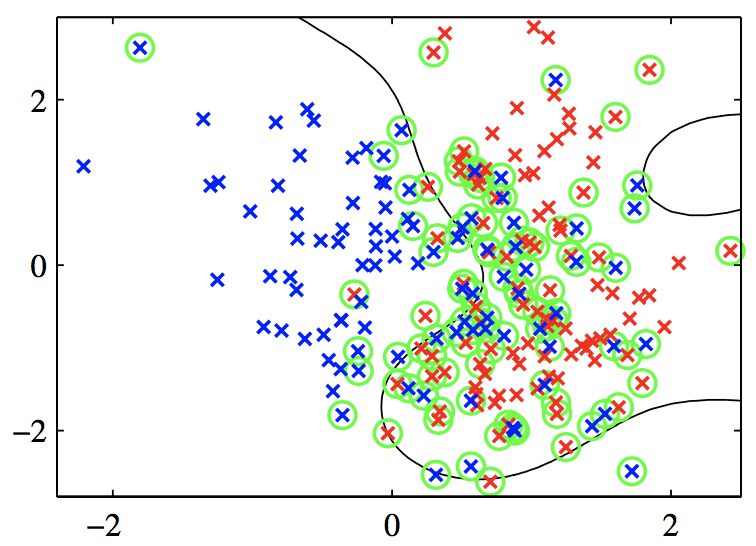
\includegraphics[scale=0.35]{svm_overlapping.png}
  \caption{
    Illustration of the $\nu$-SVM applied to a nonseparable data set in two
    dimensions.
  }
  \end{figure}
\end{frame}

\section{SVM; Regression}
\begin{frame}{SVM for regression}
  \begin{figure}
  \centering
  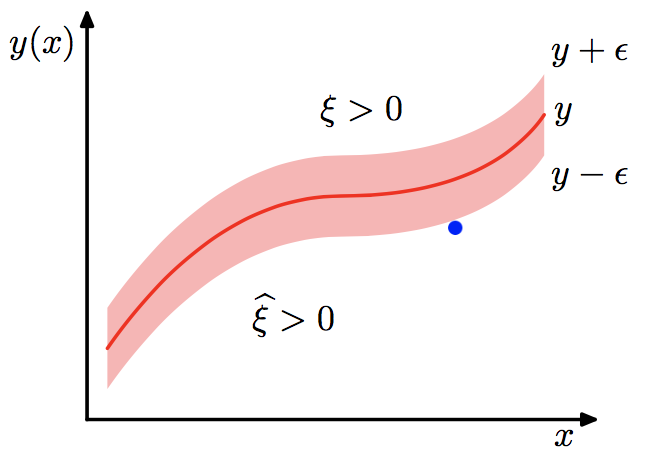
\includegraphics[scale=0.35]{svm_for_reg.png}
  \caption{
    Illustration of SVM regression.
  }
  \end{figure}
\end{frame}

\section{RVM}
\subsection{The limitations of SVM}
\begin{frame}{The limitations of SVM}
  Even though SVM have been used in a variety of classification and regression applications,
  they suffer from a number of limitations, which are given by
  \begin{itemize}
    \item \textbfit{Decision machine}; Decisions rather than posterior probabilities.
    \item originally formulated for two classes, problemetic to the extension to $K > 2$ classes.
    \item There is a \textbfit{complexity parameter} $C$, $\nu$, or even $\epsilon$ (in the case of regression),
          that must be found using a hold-out method such as cross-validation.
    \item Predictions are expressed as linear combinations of kernel functions
          that are \textbfit{centred on} training data points and
          that are required to be \textbfit{positive definite}.
  \end{itemize}

  \vspace{1.0\baselineskip}
  The \textbfit{relevance vector machine} or RVM is
  \begin{itemize}
    \item A Bayesian sparse kernel technique for regression and classification.
    \item It shares many of the characteristics of the SVM.
    \item Whilst, it avoids SVM's principal limitations.
    \item Additionally, it typically leads to much sparser models whilst
          maintaining comparable generalization error.
  \end{itemize}
\end{frame}

\begin{frame}{Model Setting}
  The model is defined by the conditional distribution for a real-valued target
  variable $t$, given an input vector $x$, which takes the form
  \begin{equation}
    \begin{gathered}
      p(t|\mathbfit{x}, \mathbfit{w}, \beta) = \mathcal{N}(t|y(\mathbfit{x}), \beta^{-1}) \\
      \textrm{where} \\
      y(\mathbfit{x}) = \sum_{i=1}^{M} w_i \phi_i (\mathbfit{x}) = \mathbfit{w}^T \boldsymbol{\phi}(\mathbfit{x})
     \end{gathered}
  \end{equation}
  Particularly, The RVM is the specific instance of this model where the basis
  functions are given by kernels, with one kernel associated with each of the
  data points from the training set, which taks the form
  \begin{equation}
    y(\mathbfit{x}) = \sum_{i=1}^{N} w_n k(\mathbfit{x}, \mathbfit{x}_n) + b
  \end{equation}
  \begin{itemize}
    \item $b$ is a bias parameter, hence the number of parameters in this case is $M = N + 1$.
    \item $y(\mathbfit{x})$ is similar with SVM's the predictive model,
          except directly using $w_i$, not $a_i$.
    \item Subsequent analysis is valid no matter what basis functions are chosen.
          For generality, we shall work with the form given in (23).
    \item No restriction: positive-definite kernel for solving optimization problem,
          choice of basis function restricted by the number or locations of training data points.
  \end{itemize}
\end{frame}

\begin{frame}{Inference stage}
  Consider the form of input as data matrix $\mathbf{X}$ and correspoinding target
  values $\mathbfsf{t}$, then the likelihood function is given by
  \begin{equation}
    p(\mathbfsf{t}|\mathbf{X}, \mathbfit{w}, \beta) =
    \prod_{n=1}^{N} \mathcal{N}(t_n | \mathbfit{w}^T \boldsymbol{\phi}(\mathbfit{x_n}), \beta^{-1}).
  \end{equation}
  Next, we introduce a prior distribution over the parameter vector $\mathbfit{w}$.
  The key difference in the RVM is that we introduce a separate hyperparameter $\alpha_i$
  for each of the weight parameter $w_i$, which takes the form
  \begin{equation}
    p(\mathbfit{w}|\boldsymbol{\alpha}) = \prod_{i=1}^{N} \mathcal{N} (w_i | 0, {\alpha_i}^{-1})
  \end{equation}
  Therefore, the posterior can be evaluated as follows
  \begin{equation}
    \begin{gathered}
      p(\mathbfit{w} | \mathbfsf{t}, \mathbf{X}, \boldsymbol{\alpha}, \beta)
      = \mathcal{N} (\mathbfit{w} | \mathbf{m}, \boldsymbol{\Sigma}) \\
      \textrm{where} \\
      \mathbf{m} = \beta \boldsymbol{\Sigma} \boldsymbol{\Phi}^T \mathbfsf{t} \\
      \boldsymbol{\Sigma} = {(\mathbf{A} + \beta \boldsymbol{\Phi}^T \boldsymbol{\Phi})}^{-1}
    \end{gathered}
  \end{equation}
  where $\boldsymbol{\Phi} = \phi_i(\mathbfit{x}_n)$ and $\mathbf{A} = \textrm{diag}(\alpha_i)$.
\end{frame}

\begin{frame}{Evidence approximation}
   The value of $\boldsymbol{\alpha}$ and $\beta$ are determined by \textbfit{evidence
   approximation},
   \begin{equation}
     p(t|\mathbfsf{t}) \simeq p(t|\mathbfsf{t},\hat{\boldsymbol{\alpha}},\hat{\beta})
     = \int p(t|\mathbfit{w}, \hat{\beta}) p(\mathbfit{w}|\mathbfsf{t},\hat{\boldsymbol{\alpha}},\hat{\beta}) \mathrm{d} \mathbfit{w}
   \end{equation}
   and then, evaluating the marginal likelihood function, we get
   \begin{equation}
     \ln p(t|\mathbfsf{t}) \simeq p(t|\mathbfsf{t},\hat{\boldsymbol{\alpha}},\hat{\beta})
     = \ln \mathcal{N} (\mathbfsf{t} | \mathbf{0}, \mathbf{C})
     = - \frac{1}{2}
     \left\{
     N \ln (2\pi) +
     \ln |\mathbf{C}| +
     \mathbfsf{t}^T \mathbf{C}^{-1} \mathbfsf{t}
     \right\}
   \end{equation}
   where $\mathbf{C} = \beta^{-1} \mathbf{I} + \boldsymbol{\Phi} \mathbf{A}^{-1} \boldsymbol{\Phi}^T$.
   Maximizing the equation with respect to $\boldsymbol{\alpha}$ and $\beta$, we
   obtain the re-estimation equations
   \begin{equation}
     \alpha_i^{(\textrm{new})} = \frac{\gamma_i}{m_i^2}
   \end{equation}
   \begin{equation}
     {\beta^{(\textrm{new})}}^{-1} = \frac{{||\mathbfsf{t} - \boldsymbol{\Phi}\mathbf{m}||}^2}{N - \sum_i \gamma_i}
   \end{equation}
   where $\gamma_i = 1 - \alpha_i \Sigma_{ii}$.
   Therefore, we shall follow this process of
   \begin{enumerate}
     \item Choosing initial value for $\boldsymbol{\alpha}$ and $\beta$.
     \item Evaluating the mean $\mathbf{m}$ and covariance $\boldsymbol{\Sigma}$ of the psoterior.
     \item Re-estimating the hyperparameters $\boldsymbol{\alpha}_{\textrm{new}}$ and $\beta_{\textrm{new}}$.
     \item Repeating re-estimation until a suitable convergence criterion is statified.
   \end{enumerate}
\end{frame}

\begin{frame}{Predictive distribution}
  Having found values $\boldsymbol{\alpha}^*$ and $\beta^*$ satisfying specific
  convergence criteria, we can evaluate the predictive distribution over $t$
  for a new input $\mathbfit{x}$ as follows
  \begin{equation}
    \begin{split}
      p(t_{\textrm{new}} | \mathbfit{x}_{\textrm{new}}, \mathbf{X}, \mathbfsf{t}, \boldsymbol{\alpha}^*, \beta^*)
      &= \int p(t|\mathbfit{x}, \mathbfit{w}, \beta^*) p(\mathbfit{w} | \mathbf{x}, \mathbfsf{t}, \boldsymbol{\alpha}^*, \beta^*) \mathrm{d}\mathbfit{w} \\
      &= \mathcal{N} (t | \mathbf{m}^T \boldsymbol{\phi}(\mathbfit{x}), \sigma^2(\mathbfit{x}))
    \end{split}
  \end{equation}
  where
  \begin{equation}
    \sigma^2(\mathbfit{x}) = \frac{1}{(\beta^*)} + {\boldsymbol{\phi}(\mathbfit{x})}^T \boldsymbol{\Sigma} \boldsymbol{\phi}(\mathbfit{x})
  \end{equation}

  In the case of an RVM with the basis functions centred on data points, the model
  will therefore become increasingly certain of its predictions when extrapolating
  outside the domain of the data, which of course is undesirable.
\end{frame}

\begin{frame}{Sparsity and Relevance Vectors}
  \textbf{The Origin of Sparsity} \\
  When we maximize the evendeince function with respect to the hpyerparameters,
  a significant proportion of $\alpha_i$ go to infinity, and the corresponding
  weight parameters $w_i$ have posterior distributions that are concentrated at
  zero, $\mathcal{N} (w_i | 0, 0)$. The basis functions associated with these
  parameters therefore play no role in the predictions made by the model and so
  are effectively pruned out, reslting in a spare model.
  \vspace{1.0\baselineskip}

  \textbf{Relevance Vector} \\
  The hyperparameters $\{\alpha_i\}$ driven to large values makes its associated
  weight parameters $w_i$ have posterior distributions $\mathcal{N} (w_i | 0, 0)$.
  Since the parameter $w_i$ is determined to be zero stritly, corresponding basis
  function $\phi_i(\mathbfit{x})$ has no role in making prediction for new inputs.
  In this casel, the input $\mathbfit{x}_n$ corresponding to the remaining nonzero
  weights are called \textbfit{relevance vectors}.

  \vspace{1.0\baselineskip}

  \textbf{Pros and Cons} \\
  We see that the number of relevance vectors in the RVM is significantly smaller
  than the number of support vectors used by the SVM, and remarkably, this greater
  sparsity is achieved with little or no reduction in generalization error compared
  with the corresponding SVM.
  The principal disadvantage of the RVM compared to the SVM is that training involves
  optimizing a nonconvex function, and training times can be longer than for a comparable SVM.
\end{frame}

\subsection{Analysis of Sparsity}
\begin{frame}{Informal insight into the origin of sparsity}
  To gett informal insight into the origin of sparsity, we are getting started
  with simpler model specified as follows
  \begin{itemize}
    \item 2 observations $t_1$ and $t_2$
    \item a signle basis $\phi(\mathbfit{x})$ with hyperparameter $\alpha$
    \item isotropic noise having precision $\beta$
    \item The marginal likelihood is given by
    $p(\mathbfsf{t} | \alpha, \beta) = \mathcal{N}(\mathbf{0}, \mathbf{C})$
  \end{itemize}
  \vspace{1.0\baselineskip}

  Then the covariance matrix of marginal likelihood function $\mathbf{C}$ is given by
  \begin{equation}
    \mathbf{C} = \frac{1}{\beta}\mathbf{I} + \frac{1}{\alpha}\boldsymbol{\varphi}\boldsymbol{\varphi}^T
  \end{equation}
  If there is poor alignment betwen the direction of $\boldsymbol{\varphi}$ and
  that of the training data vector $\mathbfsf{t}$, then the crresponding hyperparmeter
  $\alpha$ will be driven to $\infty$, and the basis vector will be pruned out from the model.
\end{frame}

\begin{frame}{General case of $M$ basis vectors (1)}
  For the more general case of $M$ basis vectors $\boldsymbol{\varphi}_m$ a similar
  intuition holds, namely that if a particular basis vector is poorly aligned with
  the data vector $\mathbfit{t}$, then it is likely to be pruned from the model.
  We now investigate this mechanism for sparsity from a more mathematical perspective.
  \vspace{1.0\baselineskip}

  At first, the re-estimation of the parameter $\alpha_i$ is given by
  \begin{equation}
    \begin{gathered}
      \alpha_i^{(\textrm{new})} = \frac{\gamma_i}{m_i^2} \\
      \textrm{where} \\
      \gamma_i = 1 - \alpha_i \Sigma_{ii}
      \quad \textrm{and} \quad
      \boldsymbol{\Sigma} = {(\mathbf{A} + \beta \boldsymbol{\Phi}^T \boldsymbol{\Phi})}^{-1}
    \end{gathered}
  \end{equation}
  \vspace{1.0\baselineskip}

  These results therefore represent implicit solutions, and iteration would be
  required even to determine a single $\alpha_i$ with all other fixed $\alpha_j$ for $j \neq i$.
\end{frame}

\begin{frame}{General case of $M$ basis vectors (2)}
  First, we pull out the contribution from $\alpha_i$ in the matrix $\mathbf{C}$ to give
  \begin{equation}
    \mathbf{C}
    = \beta^{-1} \mathbf{I}
    + \sum_{j \neq i} \alpha_j^{-1} \boldsymbol{\varphi}_j \boldsymbol{\varphi}_j^T
    + \alpha_i^{-1} \boldsymbol{\varphi}_i \boldsymbol{\varphi}_i^T
    = C_{-i} + \alpha_i^{-1} \boldsymbol{\varphi}_i \boldsymbol{\varphi}_i^T
  \end{equation}

  Using the matrix identity, the determinant and inverse of $\mathbf{C}$ can then
  be written
  \begin{equation}
    \begin{split}
      |\mathbf{C}|
      &= |\mathbf{C}_{-i}|
      (1 + \alpha_i^{-1} \boldsymbol{\varphi}_i^T \mathbf{C}_{-i}^{-1} \boldsymbol{\varphi}_i ) \\
      \mathbf{C}^{-1}
      &= \mathbf{C}_{-i}^{-1}
      - \frac{\mathbf{C}_{-i}^{-1} \boldsymbol{\varphi}_i \boldsymbol{\varphi}_i^T \mathbf{C}_{-i}^{-1} }{\alpha_i \boldsymbol{\varphi}_i^T \mathbf{C}_{-i}^{-1} \boldsymbol{\varphi}_i}
    \end{split}
  \end{equation}

  Using these results, we can separate log marginal likelihood function
  \begin{equation}
    \begin{gathered}
      L(\boldsymbol{\alpha}) = L(\boldsymbol{\alpha}_{-i}) + \lambda (\alpha_i) \\
      \textrm{where} \\
      \lambda (\alpha_i) = \frac{1}{2}
      \left[
        \ln \alpha_i - \ln(\alpha_i + s_i) + \frac{q_i^2}{\alpha_i + s_i}
      \right]
    \end{gathered}
  \end{equation}
  where the two qunatities:
  \textit{sparsity} $s_i = \boldsymbol{\varphi}_i^T \mathbf{C}_{-i}^{-1} \boldsymbol{\varphi}_i$
  and \textit{quality} $q_i = \boldsymbol{\varphi}_i^T \mathbf{C}_{-i}^{-1} \mathbfsf{t}$
\end{frame}

\begin{frame}{Sparsity and Quality}
  \begin{itemize}
    \item The sparsity $s_i$ measures the extent to which basis function $\boldsymbol{\varphi}_i$
          overlaps with the other basis vectors in the mode
    \item The quality $q_i$ represents a measure of the alignment of the basis vector
          $\boldsymbol{\varphi}_i$ with the error between the training set values $\mathbfsf{t}$
          and the vector $\mathbfsf{y}_{-i}$ of predictions that would result from
          the model with the vector $\boldsymbol{\varphi}_i$ excluded.
  \end{itemize}
  The stationary points of the marginal likelihood with respect to $\alpha_i$ occur
  when the derivative
  \begin{equation}
    \frac{\mathrm{d}}{\mathrm{d}\alpha_i} \lambda (\alpha_i)
    = \frac{\alpha_i^{-1} s_i^2 - (q_i^2 - s_i)}{2{(\alpha_i + s_i)}^2}
  \end{equation}
  is equal to zero. There are two possilble forms for the solution
  \begin{equation}
    \begin{split}
      q_i^2 < s_i &; \quad \alpha_i \rightarrow \infty \\
      q_i^2 > s_i &; \quad \alpha_i = \frac{s_i^2}{q_i^2 - s_i}
    \end{split}
  \end{equation}
  We see that the relative size of the quality and sparsity terms determines whether
  a particular basis vector will be pruned from the model or not.

  This approach
  \begin{itemize}
    \item has yielded closed-form solution for $\alpha_i$
    \item probides insight into the origin of sparsity in the RVM
    \item leads to a practical algorithm for optimizing the hyperparameters
          that has significant spped advantages.
  \end{itemize}
\end{frame}

\subsection{RVM for classification}
\begin{frame}{RVM for classification}
  To start with, we consider two-class problems with a binary target variable
  $t \in \{0, 1\}$. The model is given by
  \begin{equation}
    y(\mathbfit{x}, \mathbfit{w}) = \sigma( \mathbfit{w}^T \boldsymbol{\phi}(\mathbfit{x}))
  \end{equation}
  where $\sigma(\cdot)$ is logistic sigmoid function. We introduce Gaussian prior
  over the weight vector $\mathbfit{w}$, in which there is a separate precision hyperparameter
  associated with each weight parameter.

  Here we use the Laplace approximation, which was applied to the closely related
  problem of Bayesian logistic regression. The description of the process is given by
  \begin{enumerate}
    \item Begin with choosing initial hyperparameter $\boldsymbol{\alpha}$
    \item Given $\boldsymbol{\alpha}$, build Gaussian approximation to the
    posterior distribution and thereby an approximation to the marginal likelihood
    \item Optimize the marginal likelihood to evaluate re-estimation value of $\boldsymbol{\alpha}$
    \item repeat until convergence
  \end{enumerate}
\end{frame}
\begin{frame}{RVM for classification}
  The results are as follows
  \vspace{1.0\baselineskip}

  \textbf{re-estimation formula}
  \begin{equation}
    \alpha_i^{\textrm{new}} = \frac{\gamma_i}{{(w_i^*)}^2}
  \end{equation}
  \vspace{1.0\baselineskip}

  \textbf{Log marginal likelihood}
  \begin{equation}
    \begin{gathered}
      \ln p(\mathbfsf{t}|\boldsymbol{\alpha})
      = - \frac{1}{2}
      \left\{
      N \ln (2\pi) +
      \ln |\mathbf{C}| +
      \hat{\mathbfsf{t}}^T \mathbf{C}^{-1} \hat{\mathbfsf{t}}
      \right\} \\
      \textrm{where} \\
      \mathbf{C} = \mathbf{B} + \boldsymbol{\Phi} \mathbf{A} \boldsymbol{\Phi}^T
    \end{gathered}
  \end{equation}

  This takes the same form in the regression case, and so we can apply the same
  analysis of sparsity and obtain the same fast learning algorithm in which we
  fully optimize a single hyperparameter $\alpha_i$ at each step.
\end{frame}

\begin{frame}{RVM for classification}
  We see that the relevance vectors tend not to lie in the region of the decision
  boundary, in contrast to the support vector machine. This is consistent with our
  earlier discussion of sparsity in the RVM, because a basis function $\phi_i(\mathbfit{x})$
  centred on a data point near the boundary will have a vector $\boldsymbol{\varphi}_i$
  that is poorly aligned with the training data vector $\mathbfsf{t}$.
  \begin{figure}
  \centering
  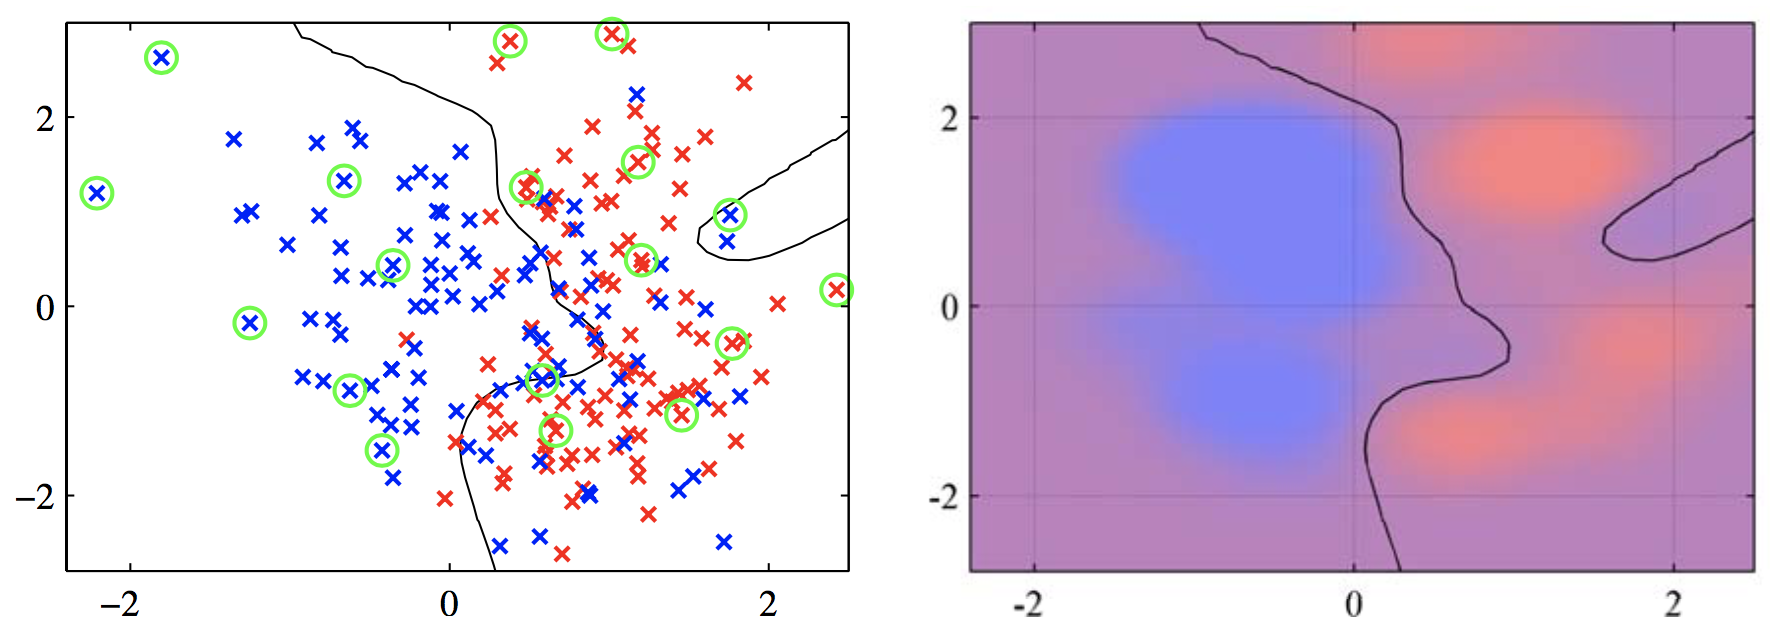
\includegraphics[scale=0.35]{rvm_classification.png}
  \caption{
    Illustration of RVM classification.
  }
  \end{figure}
\end{frame}


\begin{frame}{For $K > 2$ classes}
  $K$ linear models of the form
  \begin{equation}
    a_k = \mathbfit{w}_k^T \mathbfit{x}
  \end{equation}
  which are conbined using a softmax function to give outputs
  \begin{equation}
    y_k(\mathbfit{x}) = \frac{\exp(a_k)}{\sum_j \exp(a_j)}
  \end{equation}

  The log likelihood function is then given by
  \begin{equation}
    \ln p(\mathbf{T} | \mathbfit{w}_1, \ldots, \mathbfit{w}_K)
    = \prod_{n=1}^N \prod_{k=1}^K y_{nk}^{t_nk}
  \end{equation}
  where $t_nk$ is $1$-of-$K$ coding for each data point $n$.
\end{frame}

%%%%%%%%%%%%%%%%%%%%%%%%%%%%%%%%%%%%%%%%%%%%%%%%%%%%%%%%%%%%%%%%%%%%%
\end{document}
%%%%%%%%%%%%%%%%%%%%%%%%%%%%%%%%%%%%%%%%%%%%%%%% DOCUMENT start
